\chapter{实验结果}\label{sec:experiment}

\section{自采集数据呈现}

本项目中自采集数据分为第一次预拍摄数据Multi-Cameras1和正式拍摄数据Multi-Cameras2,两次拍摄得到的数据集与现有行人重识别领域主流数据集的比较如表\ref{tab:reiddataset}所示。我们的数据集是唯一包含大量持续跟踪行人的数据集,同一行人至少会出现在17个视野不重叠的摄像头视野内,非常适合用于要求更苛刻的行人重识别以及行人追踪任务。需要注意的是,我们现阶段统计的行人数量,只包括完整地出现在所有摄像头内的人数,而实际视频画面中还出现了很多无标签的路人,若为这些路人打上正确的标签,那么数据集中行人数量会大大增加。

\begin{table}[!htb]
\centering
\caption{行人重识别领域常见数据库情况统计}
\label{tab:reiddataset}
\begin{threeparttable}
\begin{tabularx}{\textwidth}{ccccccc}
\toprule
数据集名称   & 公布时间 & 行人数量 & 摄像头数量 & 图片数量  & Multi-shot~\tnote{a} & Tracking~\tnote{b} \\ \midrule
VIPeR\cite{gray2007evaluating}  & 2007 & 632  & 2     & 1264  & 否  & 否 \\
CUHK01\cite{li2012human} & 2012 & 971  & 2     & 3884  & 否  & 否 \\
CUHK03\cite{li2014deepreid} & 2014 & 1467 & 10    & 13164 & 是  & 否 \\
Market1501\cite{zheng2015scalable} & 2015 & 1501 & 6     & 32217 & 是  & 否 \\
DukeMTMC4reID\cite{gou2017dukemtmc4reid}  & 2017 & 1852 & 8     & 46261 & 是  & 否 \\
Multi-Cameras1 &  -~\tnote{c}   & 15~\tnote{d}   & 17     & 98543 & 是  & \textbf{是} \\
Multi-Cameras2 &  -~\tnote{c}   & 463~\tnote{d} & 24     & -~\tnote{e} & 是  & \textbf{是} \\
\bottomrule
\end{tabularx}
\begin{tablenotes}
    \footnotesize
    \item[a] 同一行人是否有超过 2 张图片。
    \item[b] 是否持续追踪同一行人。
    \item[c] 未来会公布数据库,时间待定。
    \item[d] 该数字只包含完整走完全程的演员,还有大量无标签的路人未计入。
    \item[e] 数字具体尚未统计,但预计会远大于100k。
\end{tablenotes}
\end{threeparttable}
\end{table}

\subsection{摄像头分布与分组}

表\ref{tab:cameraslayout}展示了16个摄像头的拍摄画面和分组情况。在本次采集的数据集中一共有5个场景,分别为楼外停车场、一楼庭院、二楼走廊、三楼电梯出口、三楼走廊。这5个地点分布在一条连续路线上,每个地点存在2$\sim$4个摄像头,是十分适合用于研究行人追踪的场景。

从表\ref{tab:cameraslayout}可以看出,相同拍摄地点的不同摄像头所拍摄的画面之间存在较大差异,如角度方面的差异:第2组场景一楼庭院,第1个摄像头拍摄的是行人的正背面,第2个摄像头拍摄的是行人的右俯视角度画面,第3个摄像头拍摄的是行人的左俯视角度画面。光线方面的差异:第3组场景二楼走廊,第1、4个摄像头距离行人很近,但是画面光线很暗,成像质量也很模糊,第2、3个摄像头光线较好。拍摄范围与通过时长的差异:第4组场景三楼电梯,第1、2个摄像头距离电梯门较近,行人出电梯后会在1$\sim$2秒内走出画面范围,因此相比于第3个摄像头所获得的信息相对较少。

\begin{table}[!ht]
\centering
\caption{摄像头拍摄画面及分组}
\label{tab:cameraslayout}
\renewcommand{\arraystretch}{1.5}% Spread rows out...
\begin{tabularx}{\textwidth}{>{\centering\bfseries}m{0.2\textwidth} >{\centering\arraybackslash}m{0.7\textwidth}}
\toprule
分组(场景名称) & \textbf{摄像头画面} \\
\midrule
1. 楼外停车场 & \includegraphics[width=25mm]{1-1}~\includegraphics[width=25mm]{1-2} \\
2. 一楼庭院 & \includegraphics[width=25mm]{1-4}~\includegraphics[width=25mm]{1-5}~\includegraphics[width=25mm]{1-6} \\
3. 二楼走廊 & \includegraphics[width=25mm]{2-1}~\includegraphics[width=25mm]{2-2}~\includegraphics[width=25mm]{2-3}~\includegraphics[width=25mm]{2-4} \\
4. 三楼电梯 & \includegraphics[width=25mm]{3-1}~\includegraphics[width=25mm]{3-2}~\includegraphics[width=25mm]{3-3} \\
5. 三楼走廊 & \includegraphics[width=25mm]{3-4}~\includegraphics[width=25mm]{3-5}~\includegraphics[width=25mm]{3-6}~\includegraphics[width=25mm]{3-7} \\
\bottomrule
\end{tabularx}
\end{table}

第5组场景三楼走廊也有类似情况,第1个摄像头的视野很窄,行人能够在很短时间内通过画面,而第4个摄像头则几乎能把行人通过走廊的整个过程记录下来。

\subsection{行人检测效果及人工标注结果}

行人检测使用了Detectron工具,由于Detectron实现了Mask RCNN,所以可以将行人的轮廓分割出来。图\ref{fig:detectron}展示了行人检测可视化的效果。

\begin{figure}[!ht]
\centering
\subfloat[场景1]{\centering\includegraphics[width=0.4\textwidth]{1-2_5_151}}\quad
\subfloat[场景2]{\centering\includegraphics[width=0.4\textwidth]{3-7_10_394}}\\
\subfloat[场景1检测结果]{\centering\includegraphics[width=0.4\textwidth]{1-2_5_151_det}}\quad
\subfloat[场景2检测结果]{\centering\includegraphics[width=0.4\textwidth]{3-7_10_394_det}}
\caption{Detectron行人检测结果可视化}
\label{fig:detectron}
\end{figure}

图\ref{fig:label}展示了经过人工标注后得到的同一行人在不同摄像头下的图片。从图中可以看出,同一行人在不同的视角下,差距很大,对于行人重识别算法以及人物跟踪任务极具挑战性。

\begin{figure}[!ht]
\centering
\includegraphics[width=\textwidth]{label}
\caption{同一行人在不同摄像头下的图片}
\label{fig:label}
\end{figure}\vspace{-1em}

\section{行人重识别算法}

\subsection{训练Loss曲线}

训练阶段交叉熵误差(Loss)随着数据集训练批次数(Epoch)变化曲线如图\ref{fig:loss}所示。图中共展示了第\ref{sec:modeltraining}小节所述的3个训练阶段的训练过程,每个阶段包含60个Epoch。从图中可以看出,交叉熵误差在第一训练阶段下降很明显,同时之后的测试结果\cite{sun2017beyond}也显示只使用基线模型也能达到较好的效果,说明了基线模型的稳健性。

\begin{figure}[!ht]
\centering
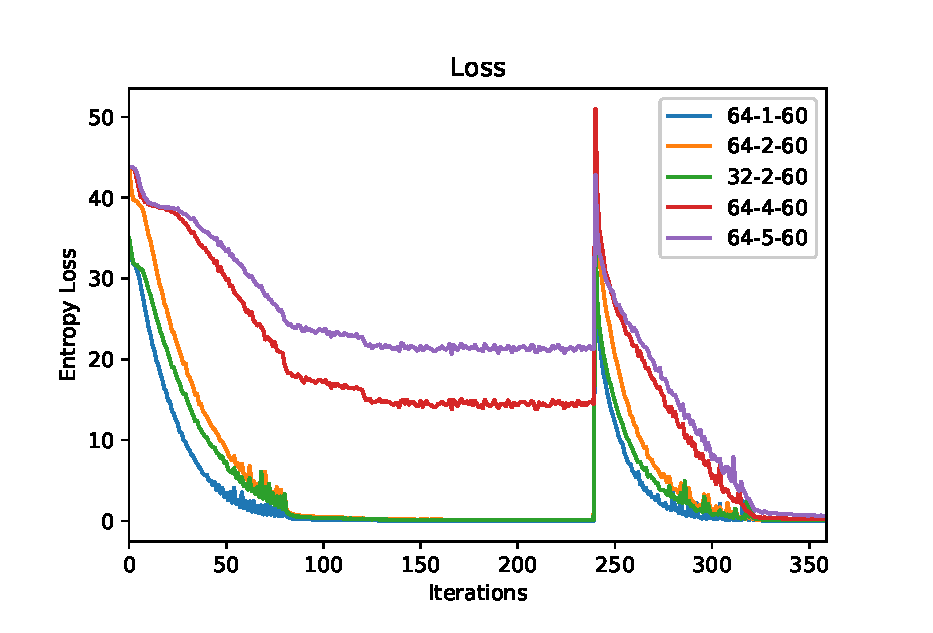
\includegraphics[width=0.6\textwidth]{loss}
\caption{交叉熵误差随着迭代次数变化曲线}
\label{fig:loss}
\end{figure}

\subsection{测试准确率比较}

表\ref{tab:test}为在Market1501测试集上的测试结果,可以看出复现的结果接近达到原论文\cite{sun2017beyond}中显示的结果。从表中可以看出,我们的PCB模型的结果以及很接近原论文中所显示的结果,但存在一个问题,我们的模型中使用RPP方法带来的提升,不及其在原论文中的表现,说明我们RPP方法的实现存在与原论文不符的情况。由于原作者尚未公布源代码,所以只能推测导致这些差异可能存在的原因:一、模型参数的初始化方式不一致,导致我们的模型与原论文中的模型收敛到了不同的局部最小值;二、不确定原始RPP模型中用于像素分类的神经网络层是否加入了Batch Normalization\cite{ioffe2015batch}层和Dropout\cite{srivastava2014dropout}层,以及它们的具体参数是多少;三、训练过程不一致,在原论文中没有清晰地说明三个训练阶段的Epoch数,以及每个训练阶段的学习率变化情况,所以只能靠人工调参。

\begin{table}[!ht]
    \centering
    \caption{Market1501数据集测试结果}
    \label{tab:test}
    \begin{threeparttable}
    \begin{tabularx}{\textwidth}{p{0.28\textwidth}p{0.2\textwidth}<{\centering}p{0.2\textwidth}<{\centering}p{0.2\textwidth}<{\centering}}
    \toprule
                            & mAP~(\%)   & Rank1~(\%) & Rank10~(\%) \\ \midrule
    PCB~(paper)~\tnote{a}    & 77.40  & 92.30  & 98.20   \\
    PCB+RPP~(paper)~\tnote{a}& 81.60  & 93.80  & 98.50   \\
    PCB                      & 73.10  & 87.20  & 93.40   \\
    PCB+RPP                  & 74.03  & 89.43  & 94.40   \\ \bottomrule
    \end{tabularx}
    \begin{tablenotes}
        \footnotesize
        \item[a] 原论文\cite{sun2017beyond}中显示的结果。
    \end{tablenotes}
    \end{threeparttable}

\end{table}

\subsection{测试结果可视化}

图\ref{fig:testvis}是行人重识别模型在Market1501数据集上测试结果的可视化,左边一列是查询图片,每一张查询图片相应的右边一行是从测试库中挑选出来的图片,有红色边框的图片代表该人物标签与相应的查询图片人物标签不一致。从图中可以看出模型的效果比较理想,仅存在少量出错的情况。同时注意到原数据库\cite{zheng2015scalable}中存在ground truth出错的情况,影响了评估指标的准确性。

\begin{figure}[!ht]
    \centering
    \includegraphics[width=0.7\textwidth]{vis3}
    \caption{测试结果可视化}
    \label{fig:testvis}
\end{figure}

\section{强化学习算法}

\subsection{学习后选择的部署方案}

表\ref{tab:rlresult}为经过强化学习训练后的智能体在应对各种状态时,最有可能采取的行动统计。其中方案~(1, 2, 7, 10, 14)~表示摄像头ID分别为1, 2, 7, 10, 14的部署方案,其它方案的表示可以此类推。表中第二列表示该方案作为其它方案的最优转移方案的频次,第三列表示该方案最优频次占方案总数的比例。

智能体经过强化学习训练,对当前环境有了了解之后,假设采用贪心的策略,即无论当前处于什么状态,都采取使得长期价值最高的动作。基于此假设,表\ref{tab:rlresult}显示,在所有可能的状态中,智能体处于其中的约$2/3$的状态下时都会一次性地转入~(1, 2, 7, 10, 14)~状态,因此该状态可以认为是智能体所选择的最优状态,该状态的可视化结果见图\ref{fig:rlresult}。处于其余约$1/3$的状态下时会转入~(1, 2, 7, 10, 13)~这个次优状态,可以看出,此方案与最优方案之间的区别,仅仅在于最后一组的摄像头的选择,而经过检查,该摄像头的成像质量也比较优秀。与此同时,当智能体处于该次优方案的状态时,长期价值最高的动作是转入最优方案状态。同时剩余的三种状态也会马上转入最优方案状态。因此可以得出结论:无论智能体当前处于什么状态,至多经过两步,即可到达最优状态。

\begin{table}[h!]
    \centering
    \caption{学习后选择的部署方案}
    \label{tab:rlresult}
    \begin{tabularx}{\textwidth}{p{0.4\textwidth}p{0.3\textwidth}p{0.3\textwidth}}
    \toprule
    方案               & 频次  & 占比~(\%)  \\ \midrule
    (1, 2, 7, 10, 14) & 190 & 65.97 \\
    (1, 2, 7, 10, 13) & 78  & 27.08 \\
    (1, 2, 7, 9, 14)  & 18  & 6.15  \\
    (1, 3, 7, 10, 14) & 1   & 0.35  \\
    (0, 2, 7, 10, 14) & 1   & 0.35  \\ \bottomrule
    \end{tabularx}
\end{table}

图\ref{fig:rlresult}是监控方案(1, 2, 7, 10, 14)的可视化结果。图中的每一张图片代表从一组摄像头中选取的一个摄像头所拍摄的场景。从图中可以看到,选取的摄像头光线充足、画面清晰、角度端正、视野范围宽阔,是一个理想的摄像头部署方案。

\begin{figure}[!ht]
    \centering
    \includegraphics[width=0.3\textwidth]{1-2}
    \includegraphics[width=0.3\textwidth]{1-4}\\
    \includegraphics[width=0.3\textwidth]{2-3}
    \includegraphics[width=0.3\textwidth]{3-2}
    \includegraphics[width=0.3\textwidth]{3-6}
    \caption{最优部署方案}
    \label{fig:rlresult}
\end{figure}

\section{分布式CPU训练}

天河二号拥有约 17920 个计算节点,每个通用节点配备两颗 Xeon E5 系列 12 核心的中央处理器、三个 XeonPhi 57 核心的协处理器(运算加速卡),总内存容量约 1.4PB,全局存储总容量约 12.4PB\cite{tianhe2018config}。2017 年 9 月,天河二号启动升级工程,二期系统天河二号 A 采用国产加速器 Matrix 2000,替换原有的 Xeon Phi 57 加速器,升级后系统峰值运算速度将达到 94.97Pflops\cite{tianhe2017summary}。天河二号各分区的详细配置如表 \ref{tab:tianheconfig}。天河二号的节点分别属于三个分区:CPU 分区、GPU 分区和胖节点分区。本项目使用了天河二号的 GPU 分区,与其它分区最大的不同在于 GPU 分区每个节点都配备了 2 块 NVIDIA Tesla K80 显示卡,显示内存 VRAM 为 24GB,单精度浮点数运算速度为 8.74 TFLOPS,双精度浮点数的运算速度为 2.91 TFLOPS。每个节点同时具备高性能的 CPU 和 GPU 运算能力,方便进行深度神经网络模型训练的对比测试。与此同时,各节点之间通过千兆网络进行连接,可用于搭建多节点分布式计算网络。

天河二号的节点分为登陆节点和计算节点。登陆节点主要用于代码编译、数据解压、环境配置等工作。计算节点配备了高性能的 CPU 和 GPU,主要用于大数据计算,以及大规模的编译任务。登陆节点和计算节点的操作系统均为 CentOS 7,系统使用 slurm 作业管理系统管理作业队列,使用 module 管理各种可选的软件包、运行库。

\begin{table}[!ht]
\centering
\caption{天河二号各分区配置表}
\label{tab:tianheconfig}
\begin{tabularx}{\textwidth}{p{0.08\textwidth}<{\centering}p{0.08\textwidth}<{\centering}p{0.35\textwidth}<{\centering}p{0.10\textwidth}<{\centering}p{0.25\textwidth}<{\centering}}
\toprule
\multicolumn{2}{c}{节点 / 分区}  & CPU                          & 内存    & GPU                  \\ \midrule
\multicolumn{2}{c}{CPU 分区}  & 2 $\times$ 12 Intel Xeon E5-2692 v2 & 64GB  & -                    \\
\multicolumn{2}{c}{GPU 分区}  & 2 $\times$ 10 Intel Xeon E5-2660 v3 & 256GB & 2 $\times$ NVIDIA Tesla K80 \\
\multirow{3}{*}{胖节点} & 128GB & 2 $\times$ 12 Intel Xeon E5-2692 v2 & 128GB & -                    \\
                        & 3TB   & 4 $\times$ 14 Intel Xeon E7-4850 v3 & 3TB   & -                    \\
                        & 6TB   & 8 $\times$ 16 Intel Xeon E7-8867 v3 & 6TB   & -                    \\ \bottomrule
\end{tabularx}
\end{table}

\subsection{多CPU集群分布式训练与单机的比较}

表\ref{tab:comp1}展示了深度行人重识别模型分别在单机及多CPU集群上训练的时间性能。第二行代表模型完整训练一个数据批次(epoch)所需的时间。从表中可以看出,采用多CPU集群取得的时间收益,与CPU节点个数近似地成线性比例关系,仅仅增加了一些节点之间通信的开销。同时,随着节点数目的增加,节点之间的通信开销也没有快速增长的趋势,说明了分布式训练的正确性和有效性。

\begin{table}[!ht]
    \centering
    \caption{多CPU集群分布式训练与单机的比较}
    \label{tab:comp1}
    \begin{threeparttable}
    \begin{tabularx}{\textwidth}{X<{\centering}X<{\centering}X<{\centering}}
    \toprule
    集群节点个数 & 时间~(~s/epoch~) & 分布式开销~(~s~)~\tnote{a} \\ \midrule
    1 & 5821 & 0   \\
    2 & 3016 & 211 \\
    4 & 1536 & 323 \\
    5 & 1219 & 274 \\ \bottomrule
    \end{tabularx}
    \begin{tablenotes}
        \footnotesize
        \item[a] 分布式开销$=$分布式训练所用时间$\times$节点个数$-$单机训练时间
    \end{tablenotes}
    \end{threeparttable}
\end{table}

\subsection{多CPU集群分布式训练与GPU的比较}

本文还将多CPU集群与单机GPU训练深度行人重识别模型进行比较,不出意外的是,单机GPU以326 s/epoch的速度将单机CPU远远甩开,按照表\ref{tab:comp1}的结果估计,大约需要包含20个节点的CPU集群才能追平GPU的速度。由此可见在运算速度上,多CPU集群不占优势。而多CPU集群相对于GPU的优势在于,其可能很轻松地拥有海量的内存,且十分容易扩展,因此可以实现同时大批量数据的运算,增大训练中的 Batch Size,使得模型参数的梯度计算更加准确,从而可以使用更大的学习率。与此同时,根据Smith等人\cite{smith2017don}的研究,在训练过程中动态地增加Batch Size,可以代替动态地衰减学习率。使用大的学习率,可以加速模型参数的收敛,因此训练模型可以经历更少的Epoch,达到加速训练的目的。

表\ref{tab:comp2}是多CPU集群(包含5个CPU节点)与GPU在训练深度行人重识别模型时,不同的Batch Size、学习率、Epoch数以及准确率的比较。

\begin{table}[h!]
    \centering
    \caption{多CPU集群分布式训练与GPU的比较}
    \label{tab:comp2}
    \begin{threeparttable}
    \begin{tabularx}{\textwidth}{X<{\centering}X<{\centering}X<{\centering}X<{\centering}X<{\centering}X<{\centering}}
    \toprule
    模型    & Batch Size & 学习率~\tnote{a} & Epoch数 & 训练时间~(s) & Rank1~(\%)  \\ \midrule
    GPU     & 48 & 0.1 & 60 & - & 89.43 \\
    CPU集群1 & 128 & 0.5 & 40 & - & - \\
    CPU集群2 & 256 & 1.0 & 30 & - & - \\
    CPU集群3 & 512 & 2.0 & 20 & - & - \\
    CPU集群4 & 768 & 3.0 & 10 & - & - \\ \bottomrule
    \end{tabularx}
    \begin{tablenotes}
        \footnotesize
        \item[a] 初始的基准学习率
    \end{tablenotes}
    \end{threeparttable}
\end{table}